\PassOptionsToPackage{implicit=true}{hyperref}
\documentclass[10pt, aspectratio=169, compress, protectframetitle, handout]{beamer}

\usepackage{iftex}
\ifxetex
    \usepackage{fontspec}
\else
    \usepackage[T1]{fontenc}
    \usepackage[utf8]{inputenc}
\fi
\usepackage[english]{babel}
\usepackage{appendixnumberbeamer}
% handout to deactivate \uncover
% usetitleprogressbar might be needed
%\usepackage{beamerprosper}
\usepackage{comment}
% Load BEFORE the theme
\usepackage[normalem]{ulem}

\usetheme[progressbar=frametitle,block=fill,numbering=fraction]{metropolis}
\setbeamertemplate{blocks}[rounded][shadow=true]

% Change Colors/Width of Progress Bars 
\makeatletter
%\setlength{\metropolis@titleseparator@linewidth}{1pt}
\setlength{\metropolis@progressonsectionpage@linewidth}{0.8pt}
\setlength{\metropolis@progressinheadfoot@linewidth}{1pt}
\makeatother

%\setbeamertemplate{note page}[plain]
%\setsansfont[
%     Extension      = .otf,
%     UprightFont    = *-Light,
%     ItalicFont     = *-LightItalic,
%     BoldFont       = *-Regular,
%     BoldItalicFont = *-RegularItalic
% ]{FiraSans}
%\setmonofont[
%     Extension   = .otf,
%     UprightFont = *-Regular,
%     BoldFont    = *-Medium
%]{FiraMono}


\newcommand{\putbg}{\usebackgroundtemplate{
\includegraphics[width=\paperwidth,height=\paperheight]{background-vector_169}}}
\newcommand{\putbgdark}{\usebackgroundtemplate{
\includegraphics[width=\paperwidth,height=\paperheight]{background-vector-dark_169}}}


\usepackage[export]{adjustbox}
\usepackage[]{enumitem}
\usepackage{datetime}
\usepackage{textpos}
\usepackage{xcolor}
\usepackage{marvosym} % Smile
\usepackage{fontawesome5} % Icons
\usepackage{wrapfig} % To wrap figures wih text
%\usepackage{cleveref} % To fix autoref links not working
\usepackage{subcaption}
\usepackage{csquotes}

\mathchardef\mhyphen="2D % dash in math mode

% Fixes bad positioning of hats
\usefonttheme{professionalfonts}%[onlymath]{serif}
\PassOptionsToPackage{hyphens}{url}\usepackage{hyperref} % to break the links
\hypersetup{
    colorlinks = true,
    linkcolor  = ,       % color of internal links
    urlcolor   = blue,   % color of external links
    pdftitle   = {Master\_Thesis\_Slides},
    pdfauthor  = {Angela Carraro}
}


%%%%%%%%%%%%%%%%%%%%%%%%%%%%%%%%%%%%%%%%%%%%%%%%%%%%%%%%%%%
% TITLE FRAME                                             %
%%%%%%%%%%%%%%%%%%%%%%%%%%%%%%%%%%%%%%%%%%%%%%%%%%%%%%%%%%%
% https://tex.stackexchange.com/questions/478172/metropolis-beamer-title-page

\setbeamertemplate{title page}{
  \begin{minipage}[b][\paperheight]{\textwidth}
    \ifx\inserttitlegraphic\@empty\else\usebeamertemplate*{title graphic}\fi
    \vspace*{0.5cm}
    \vfill%
    \ifx\inserttitle\@empty\else\usebeamertemplate*{title}\fi
    \ifx\insertsubtitle\@empty\else\usebeamertemplate*{subtitle}\fi
    \usebeamertemplate*{title separator}
    \begin{minipage}[t]{0.5\textwidth}
		    { \normalsize \scshape Candidate: }\\
			{ \small \THauthor } \\[0.10cm]
			{ \normalsize \scshape Supervisor: }\\
			{ \small \THsupervisor }
	\end{minipage}
	\hspace*{1cm}
	\begin{minipage}[t]{0.5\textwidth}
            { \normalsize \scshape Co-Supervisors: }\\[0.10cm]
			{ \small \THcosupervisor }\\[0.10cm]
			{ \small \THextracosupervisor }\\[0.10cm]
			{ \small \THextracosupervisortwo }
    \end{minipage}
    \vfill%
	\begin{minipage}[t]{\textwidth}
        \ifx\insertinstitute\@empty\else\usebeamertemplate*{institute}\fi
    \end{minipage}
    \vfill%
    \vspace*{1pt}
  \end{minipage}
}


%%% Metadati
\graphicspath{{figures/PNG/}{figures/PDF/}{figures/}}
\newdateformat{monthyear}{\monthname[\THEMONTH] \THEYEAR}
\title{Optimizing fault search in power grid outages through Reinforcement Learning}
\subtitle{Master's degree in \emph{Data Science and Scientific Computing}}
\def\THauthor{Angela Carraro}
\def\THsupervisor{Antonio Celani, ICTP}
\def\THcosupervisor{Andrea Zancola, AcegasApsAmga}
\def\THextracosupervisor{Luca Bortolussi, UniTS}
\def\THextracosupervisortwo{Emanuele Panizon, ICTP}
\date{}
\institute{\footnotesize \scshape DSSC - UniTS, SISSA, ICTP\\
\vfill

\includegraphics[valign=c, height=0.7cm]{logo_dssc_alt}
\hspace*{0.5cm}

\includegraphics[valign=c, height=0.75cm]{Logo_units_blu}
\hspace*{0.5cm}

\includegraphics[valign=c, height=0.74cm]{International_Centre_for_Theoretical_Physics.png}
\hspace*{0.5cm}

\includegraphics[valign=c, height=0.75cm]{SISSA_official_logo_2019_ALT.pdf}
}

\addtobeamertemplate{frametitle}{}{%
\begin{textblock*}{100mm}(0.90\textwidth,-0.94cm)

\includegraphics[valign=c, height=0.4cm]{logo_dssc_alt_white}

\includegraphics[valign=c, height=0.45cm]{Logo_units_white}
\end{textblock*}}


\begin{document}

{\putbg\maketitle}

\begin{frame}{Aim of the project}

    \bigskip\bigskip

    \begin{displayquote}
        \large
        We want to \alert{optimize the fault search} in power grid outages through \alert{Reinforcement learning}.
    \end{displayquote}
    
    \vspace*{20pt}
    
    \alert{Why?}
    \begin{itemize}
        \item[\alert{$\bullet$}] The restoration process is done by the technicians using only their experience.
        \medskip
        \item[\alert{$\bullet$}] We want to exploit the data on the power grid that we have at our disposal.
    \end{itemize}
    
\end{frame}

{\putbg
\section{The restoration process}
}

\begin{frame}{Example of a power line in medium voltage}
    \vspace{-5pt}
    \begin{figure}
        \centering
        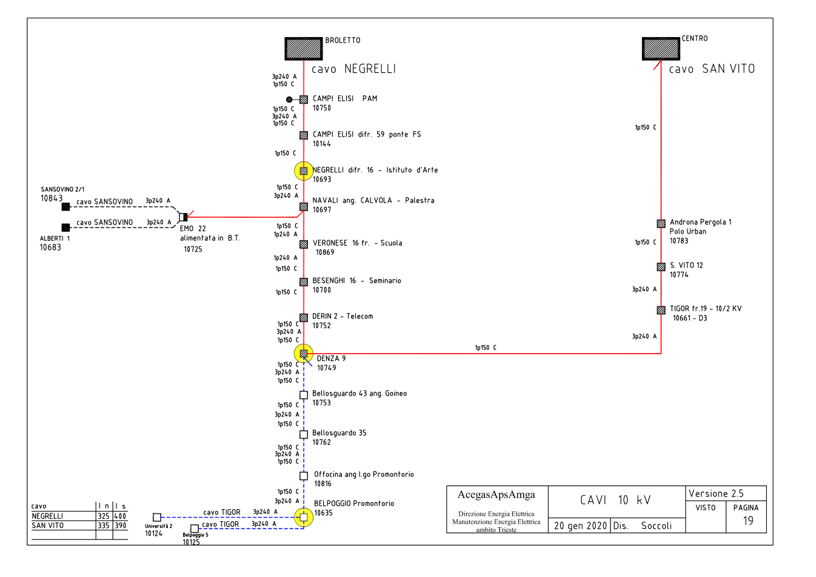
\includegraphics[width=0.8\textwidth]{figures/Rete_TS_1.png}
    \end{figure}
\end{frame}

\begin{frame}{The energy flow in the standard set-up}
    \vspace{-5pt}
    \begin{figure}
        \centering
        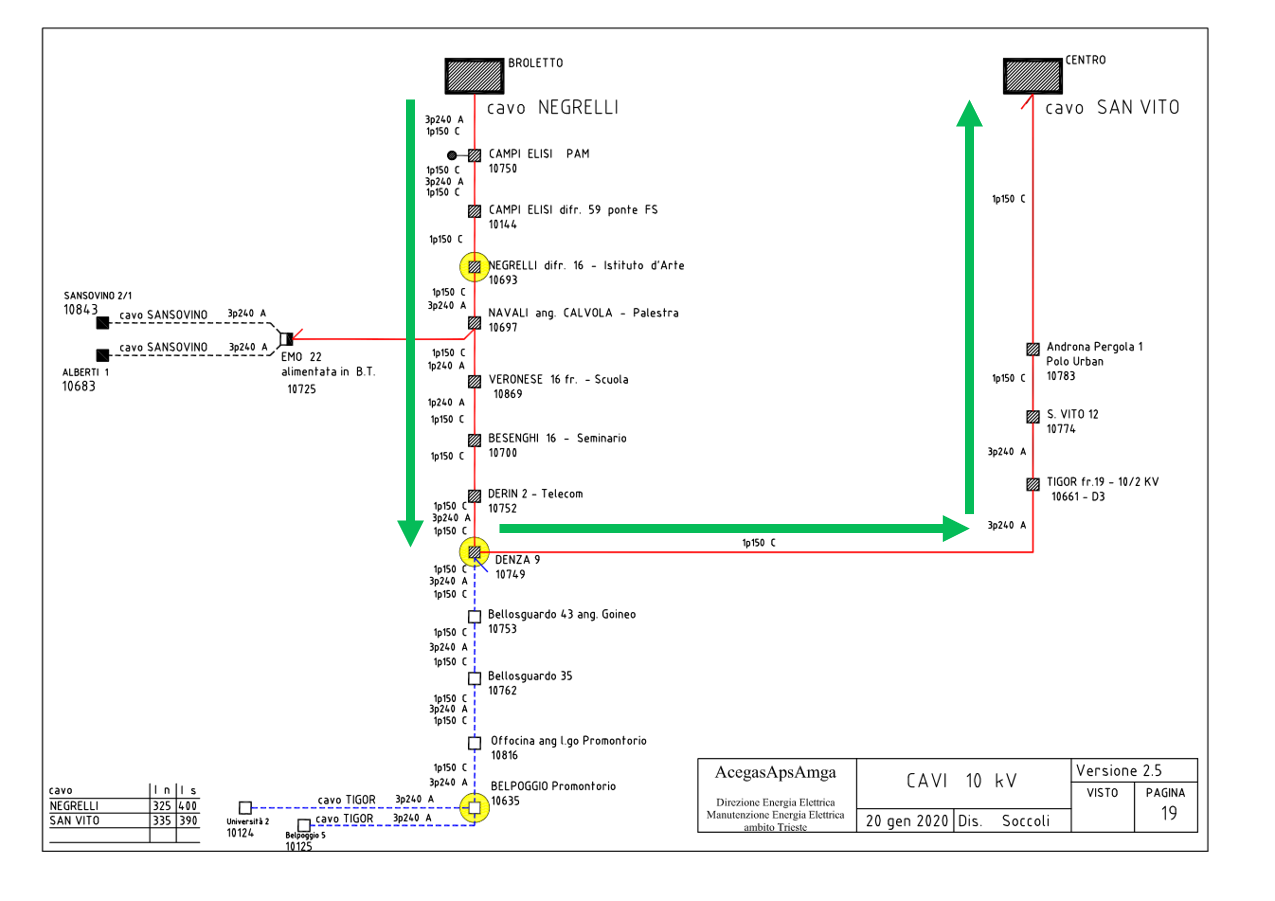
\includegraphics[width=0.8\textwidth]{figures/Rete_TS_2.png}
    \end{figure}
\end{frame}

\begin{frame}{Failure scenario}
    \vspace{-5pt}
    \begin{figure}
        \centering
        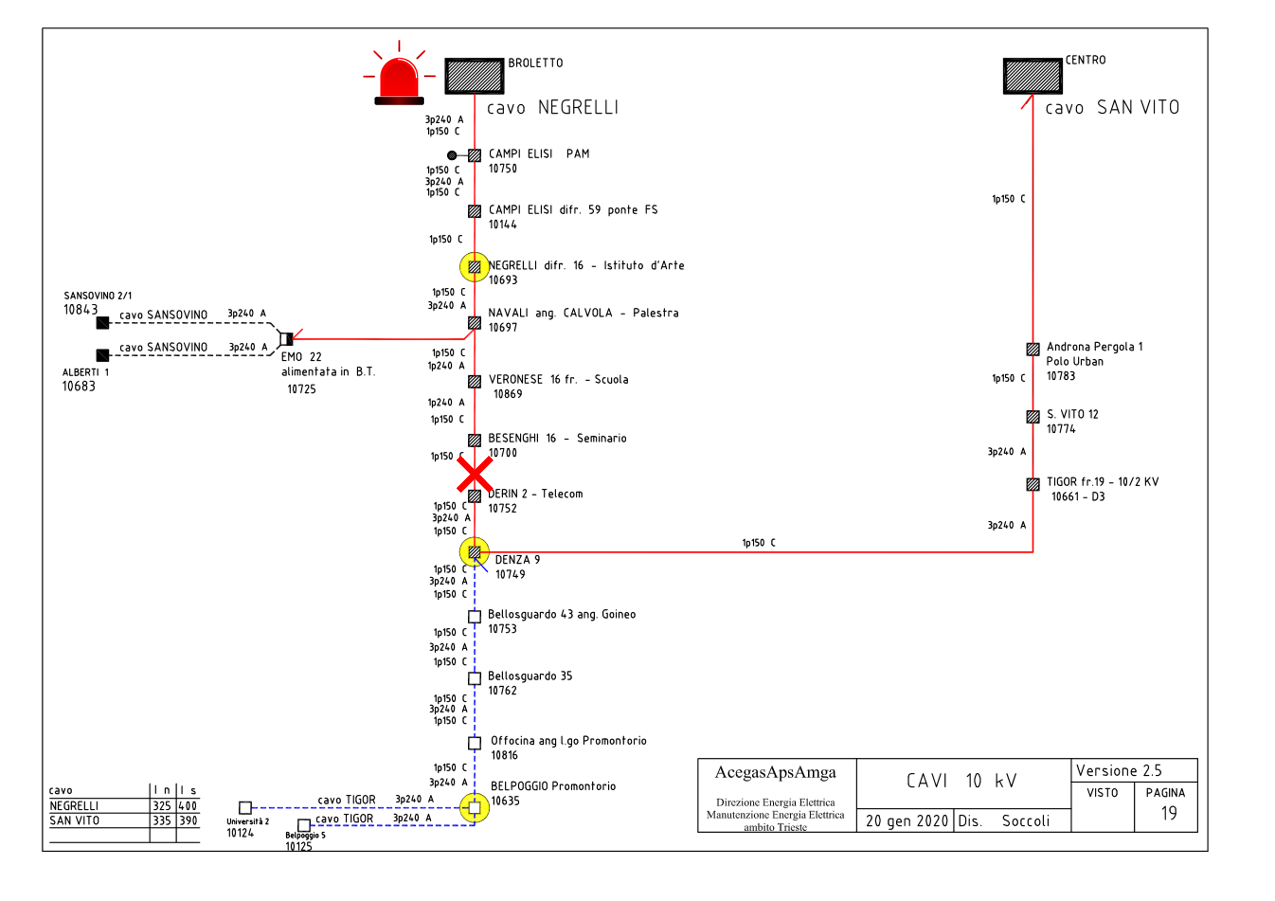
\includegraphics[width=0.8\textwidth]{figures/Rete_TS_3.png}
    \end{figure}
\end{frame}

\begin{frame}{Failure scenario}
    \vspace{-5pt}
    \begin{figure}
        \centering
        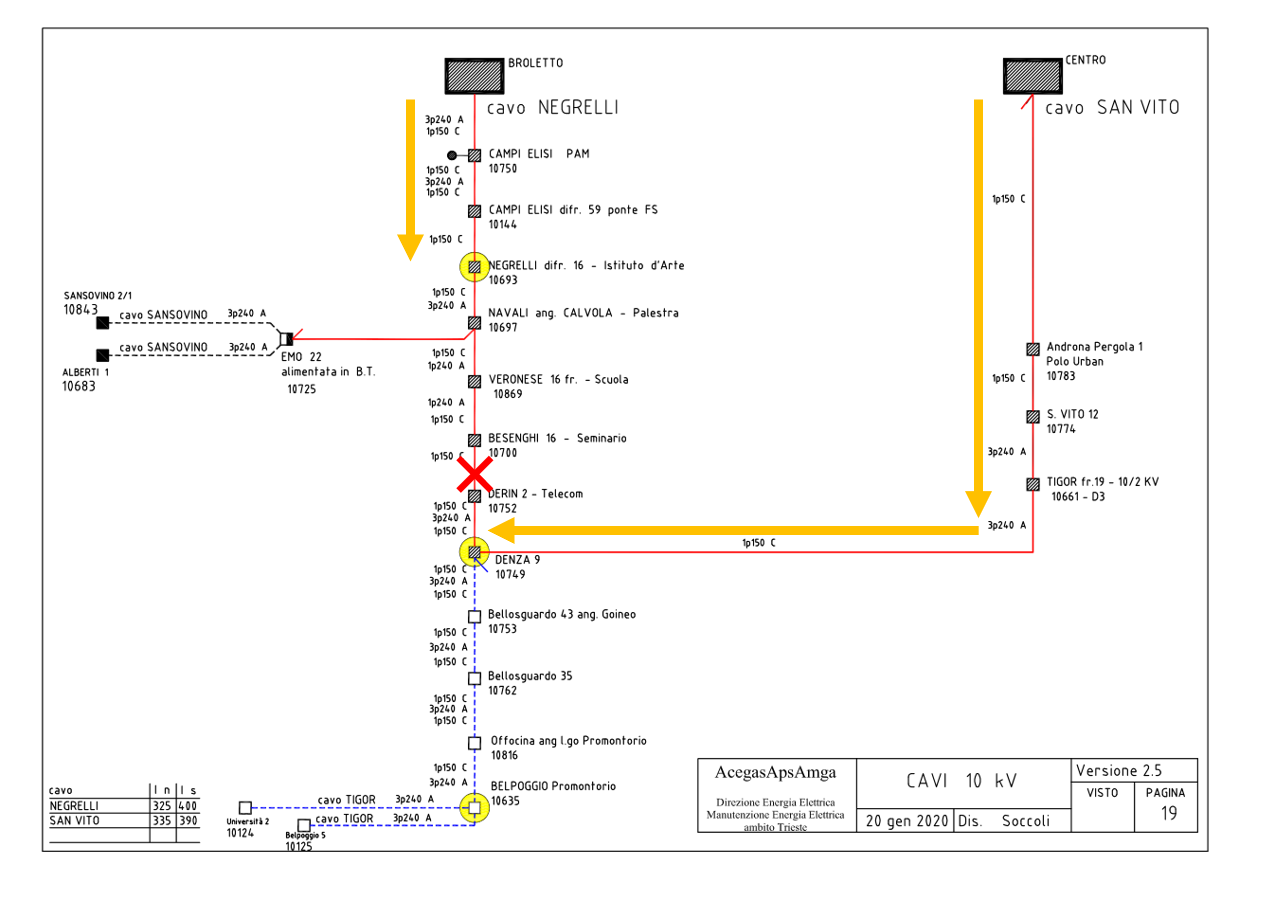
\includegraphics[width=0.8\textwidth]{figures/Rete_TS_4.png}
    \end{figure}
\end{frame}

\begin{frame}{Failure scenario}
    \vspace{-5pt}
    \begin{figure}
        \centering
        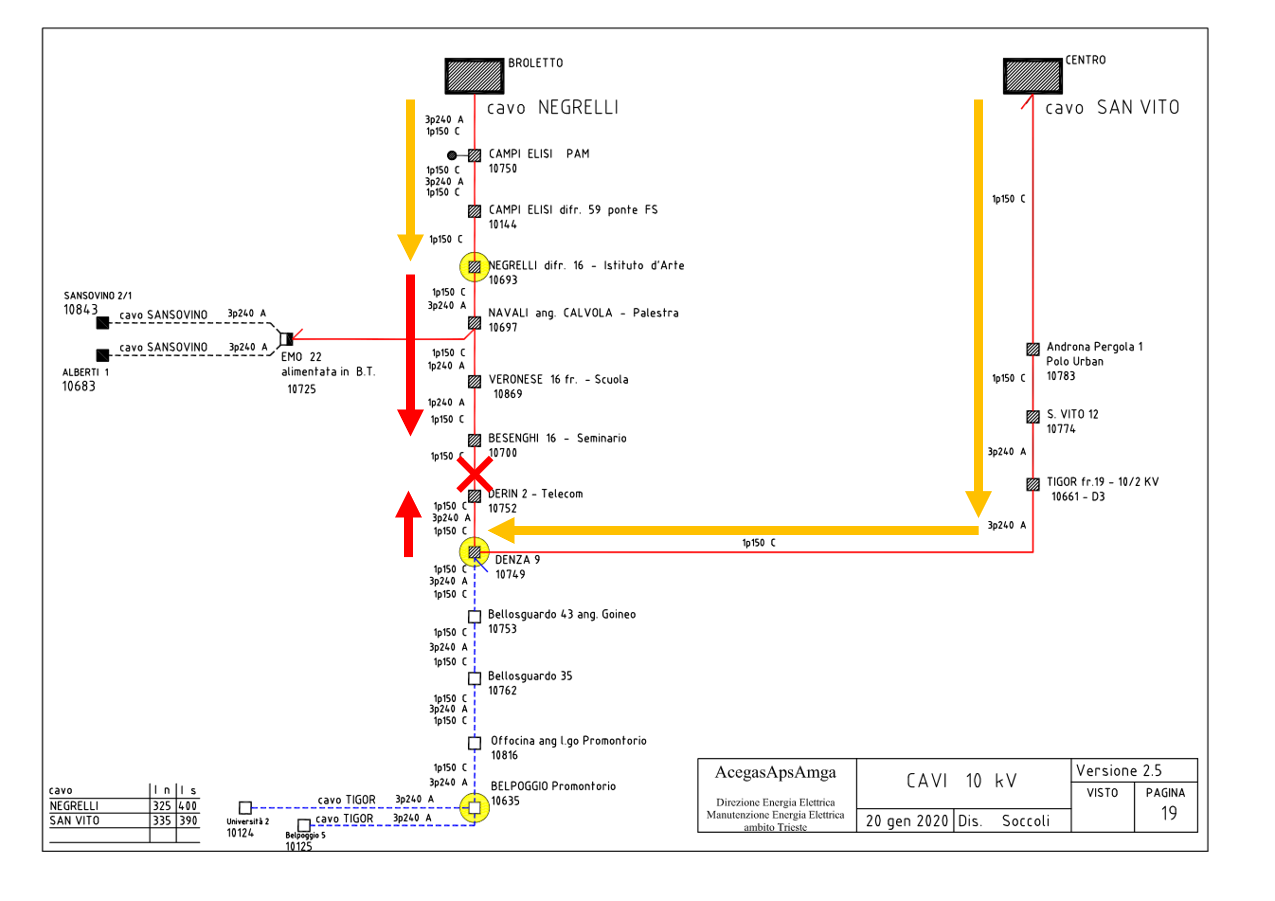
\includegraphics[width=0.8\textwidth]{figures/Rete_TS_5.png}
    \end{figure}
\end{frame}

{\putbg
\section{The mathematical model}
}

\begin{frame}{Reinforcement Learning}

    At the beginning, we are given a set of disconnected substations, $\mathcal C$, between two remotely controlled substations.
    \bigskip

    \begin{columns}[onlytextwidth]
        \begin{column}{.6\textwidth}
            To model the problem, we used a \alert{partially observable Markov decision process (POMDP)}, since we don't know where the fault is. In this model, we have an \alert{agent} in an \alert{environment}, and the former has to take \alert{actions} according to a \alert{policy} $\pi$ to minimize the \alert{expected cost} $J$.
        \end{column}
        \begin{column}{.4\textwidth}
            \vspace*{-15pt}
            \begin{figure}
                \centering
                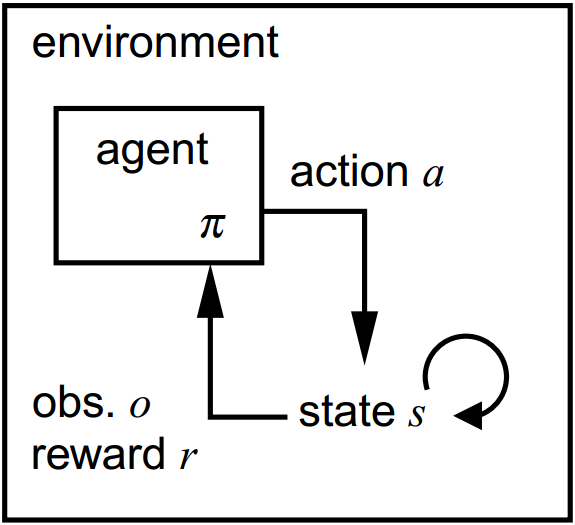
\includegraphics[width=3.5cm]{figures/POMDP-schema.png}
            \end{figure}
        \end{column}
    \end{columns}
    \medskip

    In our specific problem, the \alert{action} is the choice of the specific substation the technician will visit as the next step.
    
    Instead, the \alert{expected cost} is the time (\textit{in seconds}) of going to a certain substation multiplied by the number of disconnected users.
    
\end{frame}

\begin{frame}{Our algorithms}

    We use the \alert{Policy Gradient (PG) algorithm}, in which we \textbf{parametrize the policy} and we try to find the best policy in order to optimize the POMDP.
    
    \textit{How do we do it?} \textbf{We start from a certain policy}, for example the \emph{random policy}, in which all actions have an equal probability of being selected. Then we \textbf{perform gradient descent on the parameters of the policy}.
    
    This algorithm has a \textbf{very slow convergence}, so we also implemented the \alert{Natural Policy Gradient (NPG) algorithm}, which only changes the formula of the gradient to speed up convergence.
    
\end{frame}

{\putbg
\section{Results}
}

\begin{frame}{Convergence times of PG and NPG}

    \begin{figure}
        \centering
        \mbox{
            \hspace*{-15pt}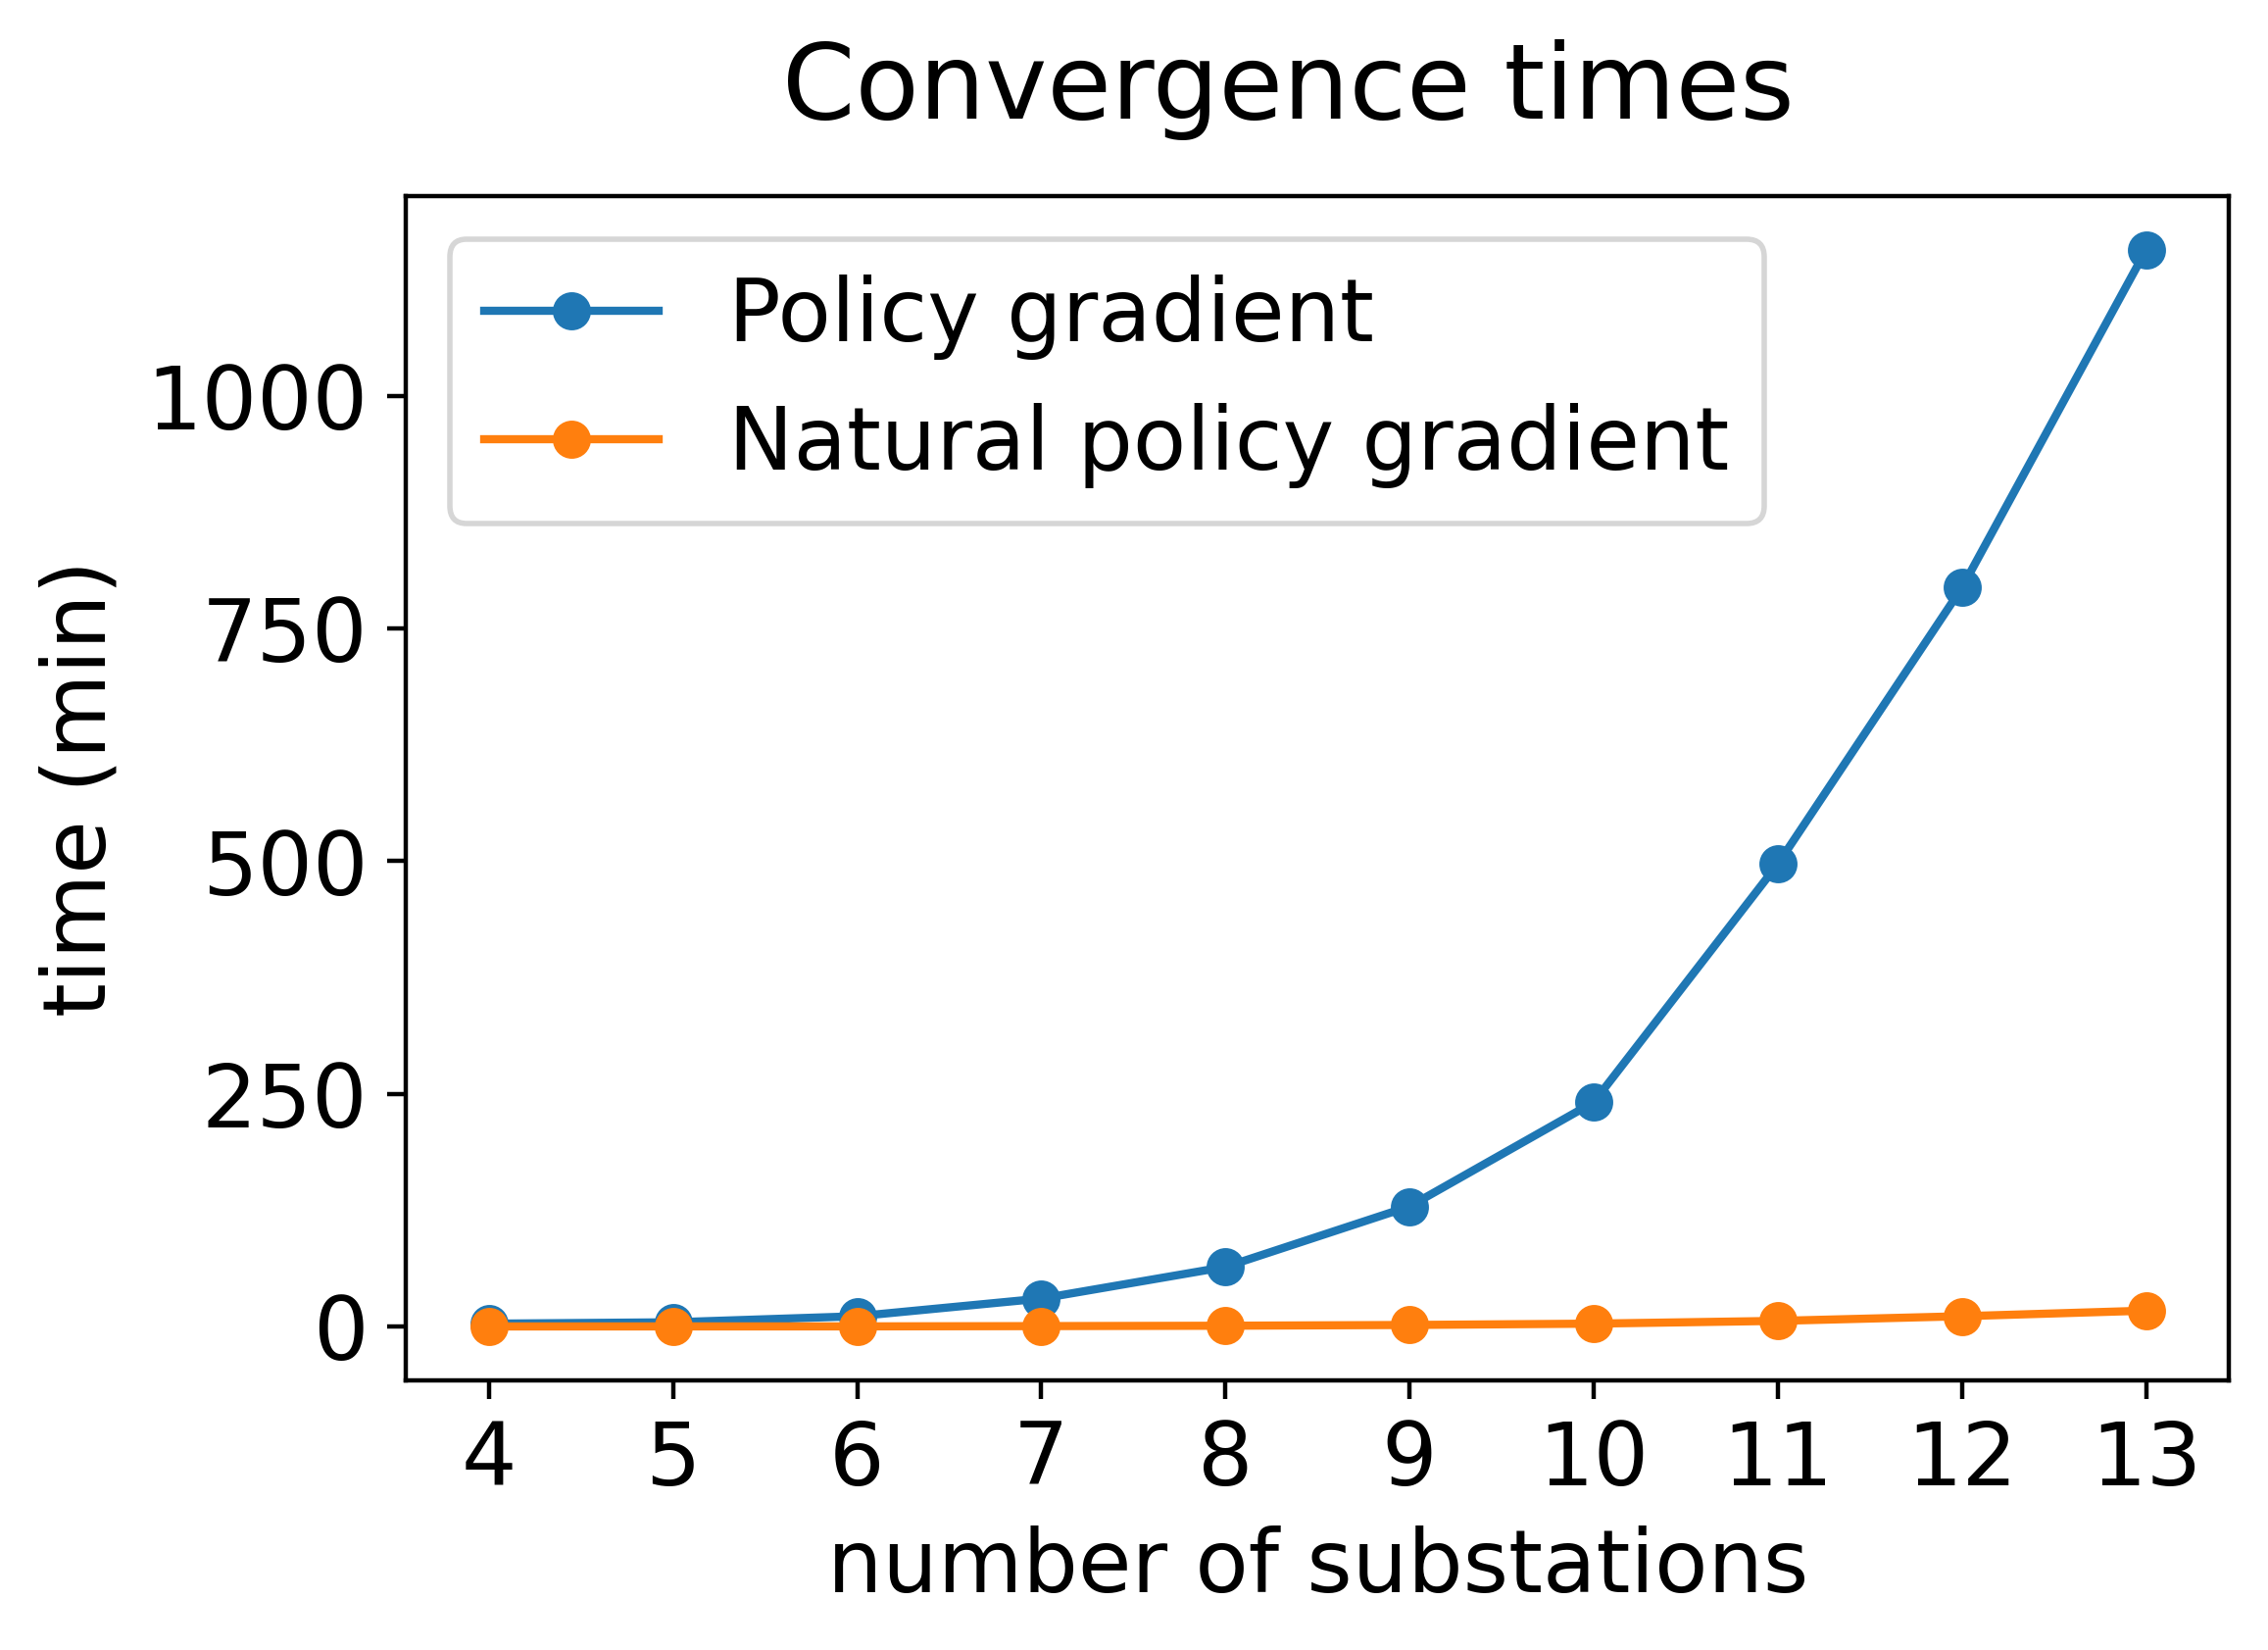
\includegraphics[scale=0.5]{figures/times_graph.png}
            \hspace*{-5pt}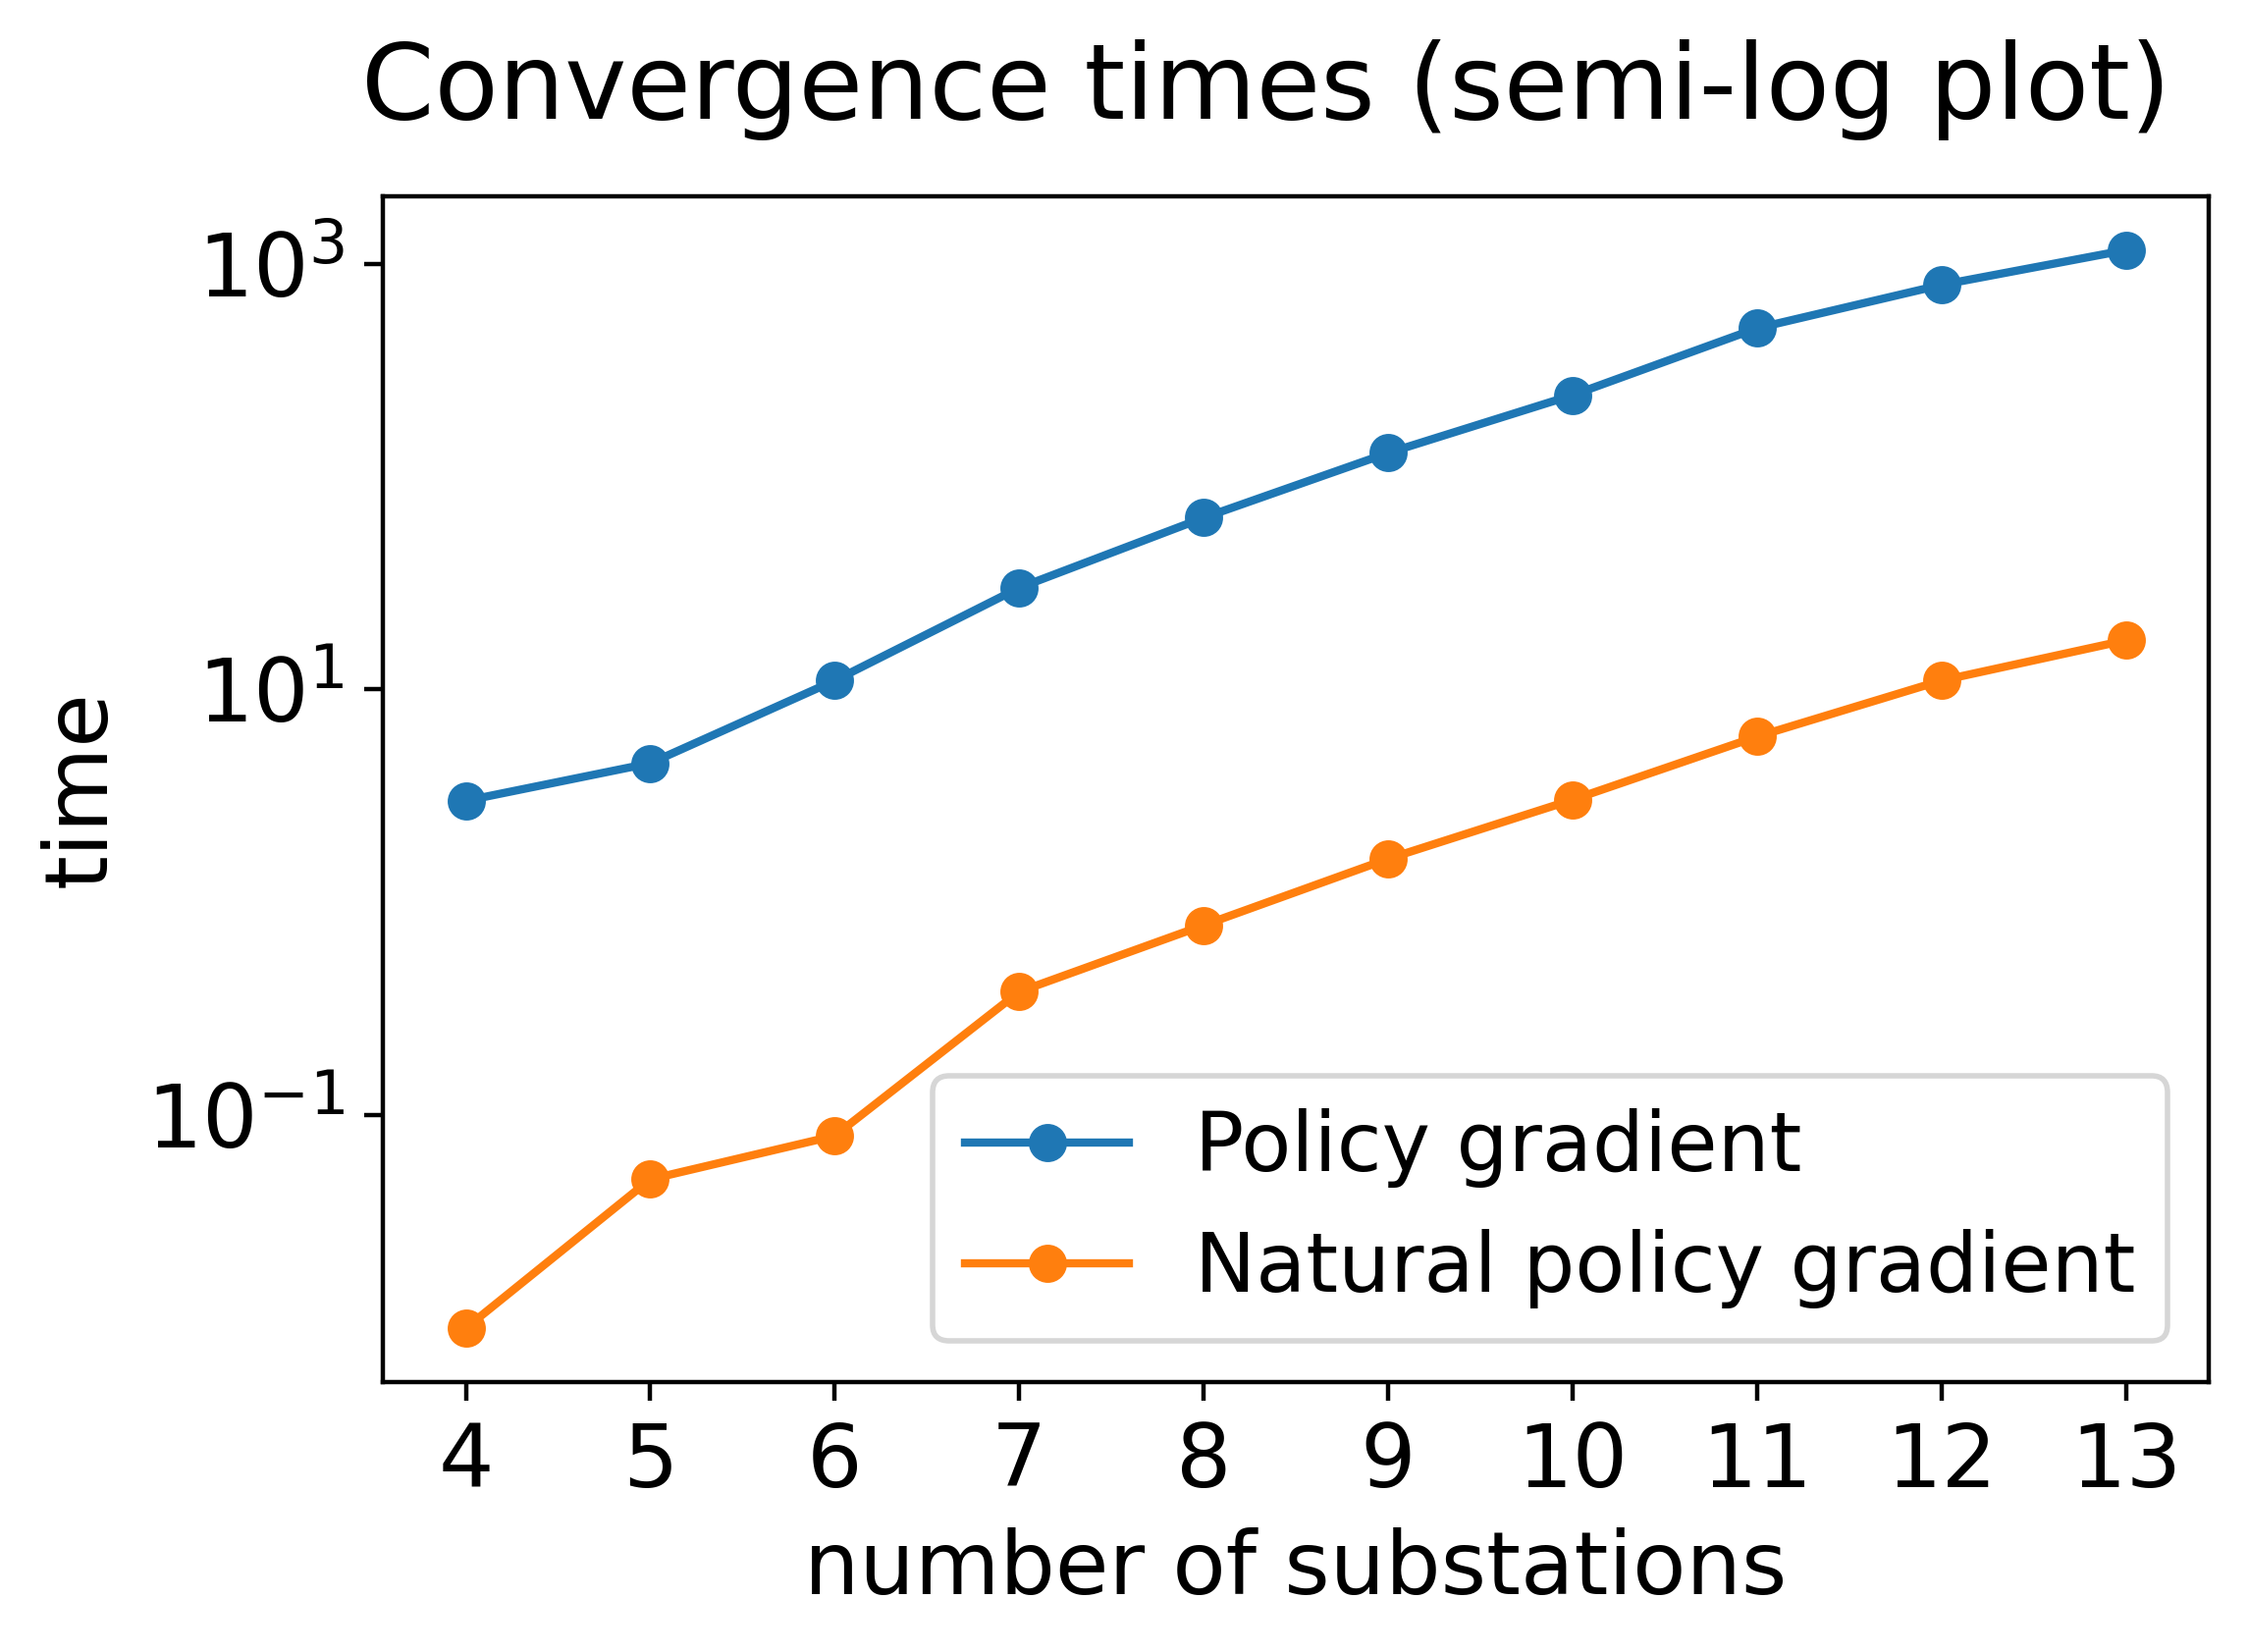
\includegraphics[scale=0.5]{figures/times_graph_log.png}
        }
    \end{figure}
    
\end{frame}

\begin{frame}{}

    \begin{figure}
        \centering
        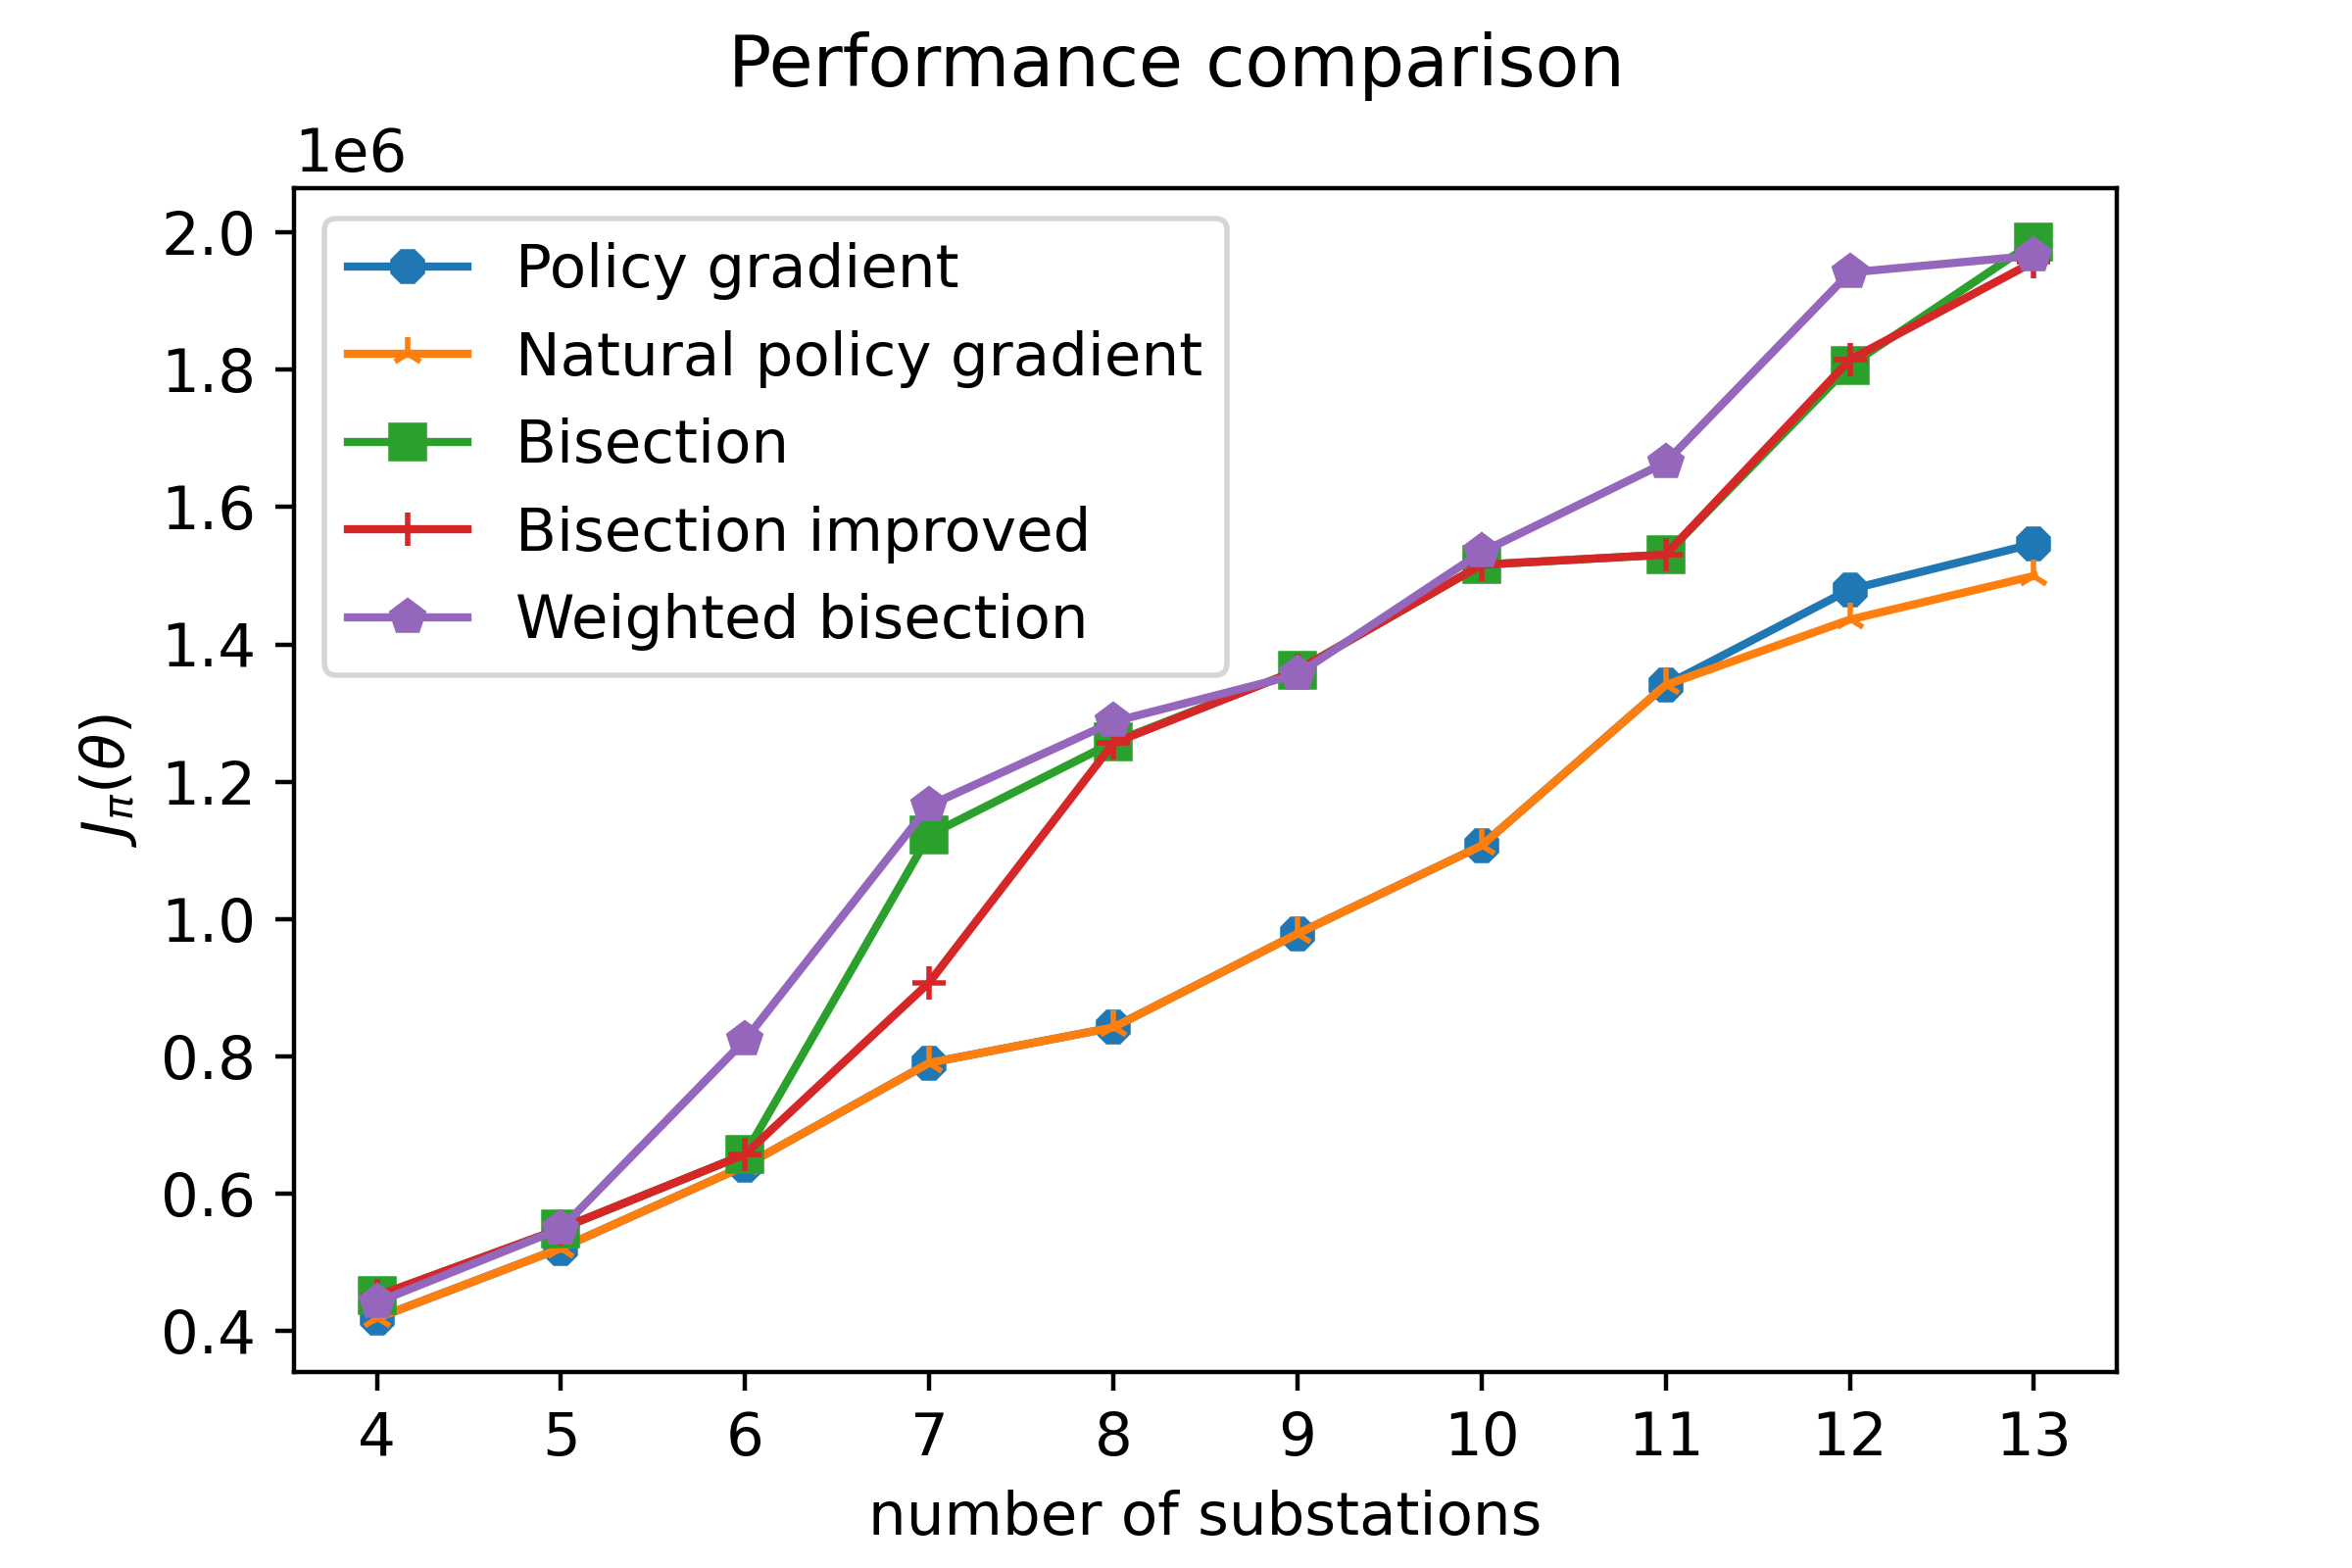
\includegraphics[scale=0.85]{figures/comparison_graph.png}
    \end{figure}
    
\end{frame}

\begin{frame}{Recap}

    Thus, we optimized the fault search in power grid outages:

    \begin{itemize}
        \item[\alert{$\bullet$}] We modeled Trieste's power grid using \alert{graphs}.
        \item[\alert{$\bullet$}] We modeled the current method used by the technicians to find the fault during the restoration process: the \alert{bisection} algorithm.
        \item[\alert{$\bullet$}] We developed a new algorithm that was able to exploit the data that we have on the substations and to improve the restoration process: the \alert{(natural) policy gradient} algorithm.
    \end{itemize}
    
\end{frame}

{\putbgdark
\begin{frame}[standout]
	\begin{center}
		\Large \uncover<+->{Thank you for your attention!}
		
		\Huge\uncover<+->{\Smiley}
	\end{center}
\end{frame}
}

{\putbg
\section{Backup slides}
}

\begin{frame}[noframenumbering]{}

    \begin{figure}
        \centering
        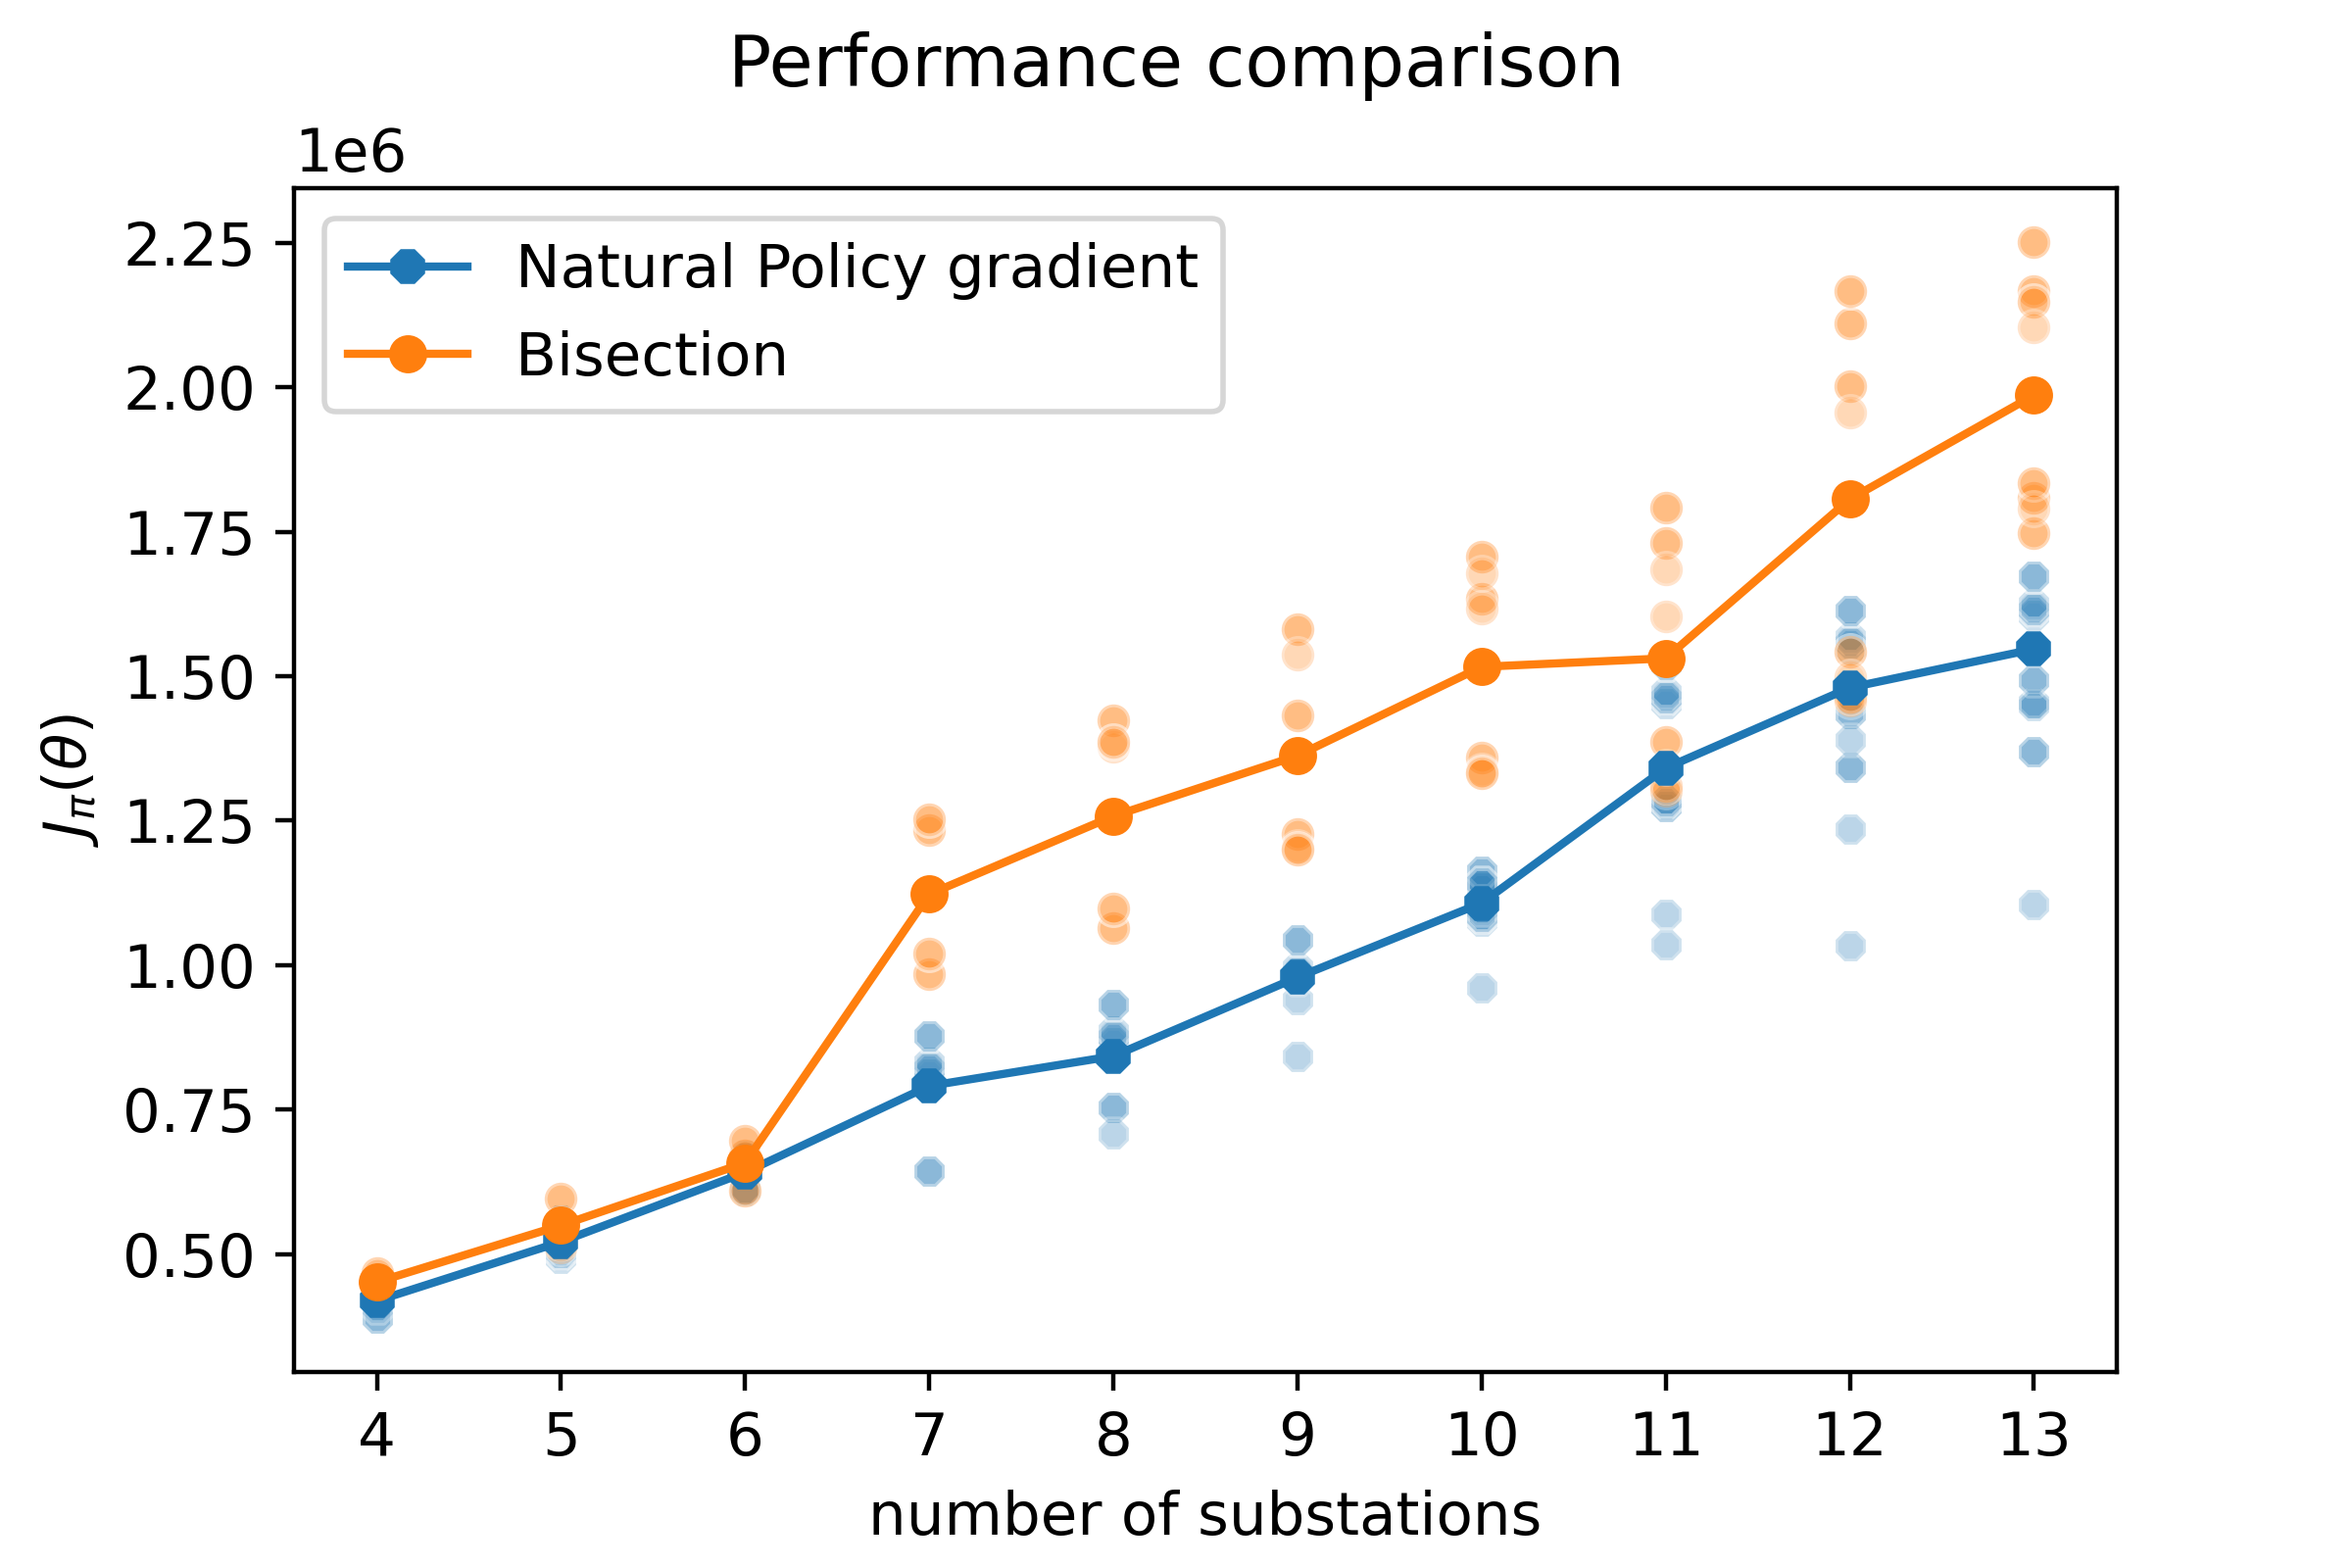
\includegraphics[scale=0.85]{figures/comparison_graph_scatterplot.png}
    \end{figure}
    
\end{frame}

\begin{frame}[noframenumbering]{}

    \begin{figure}
        \centering
        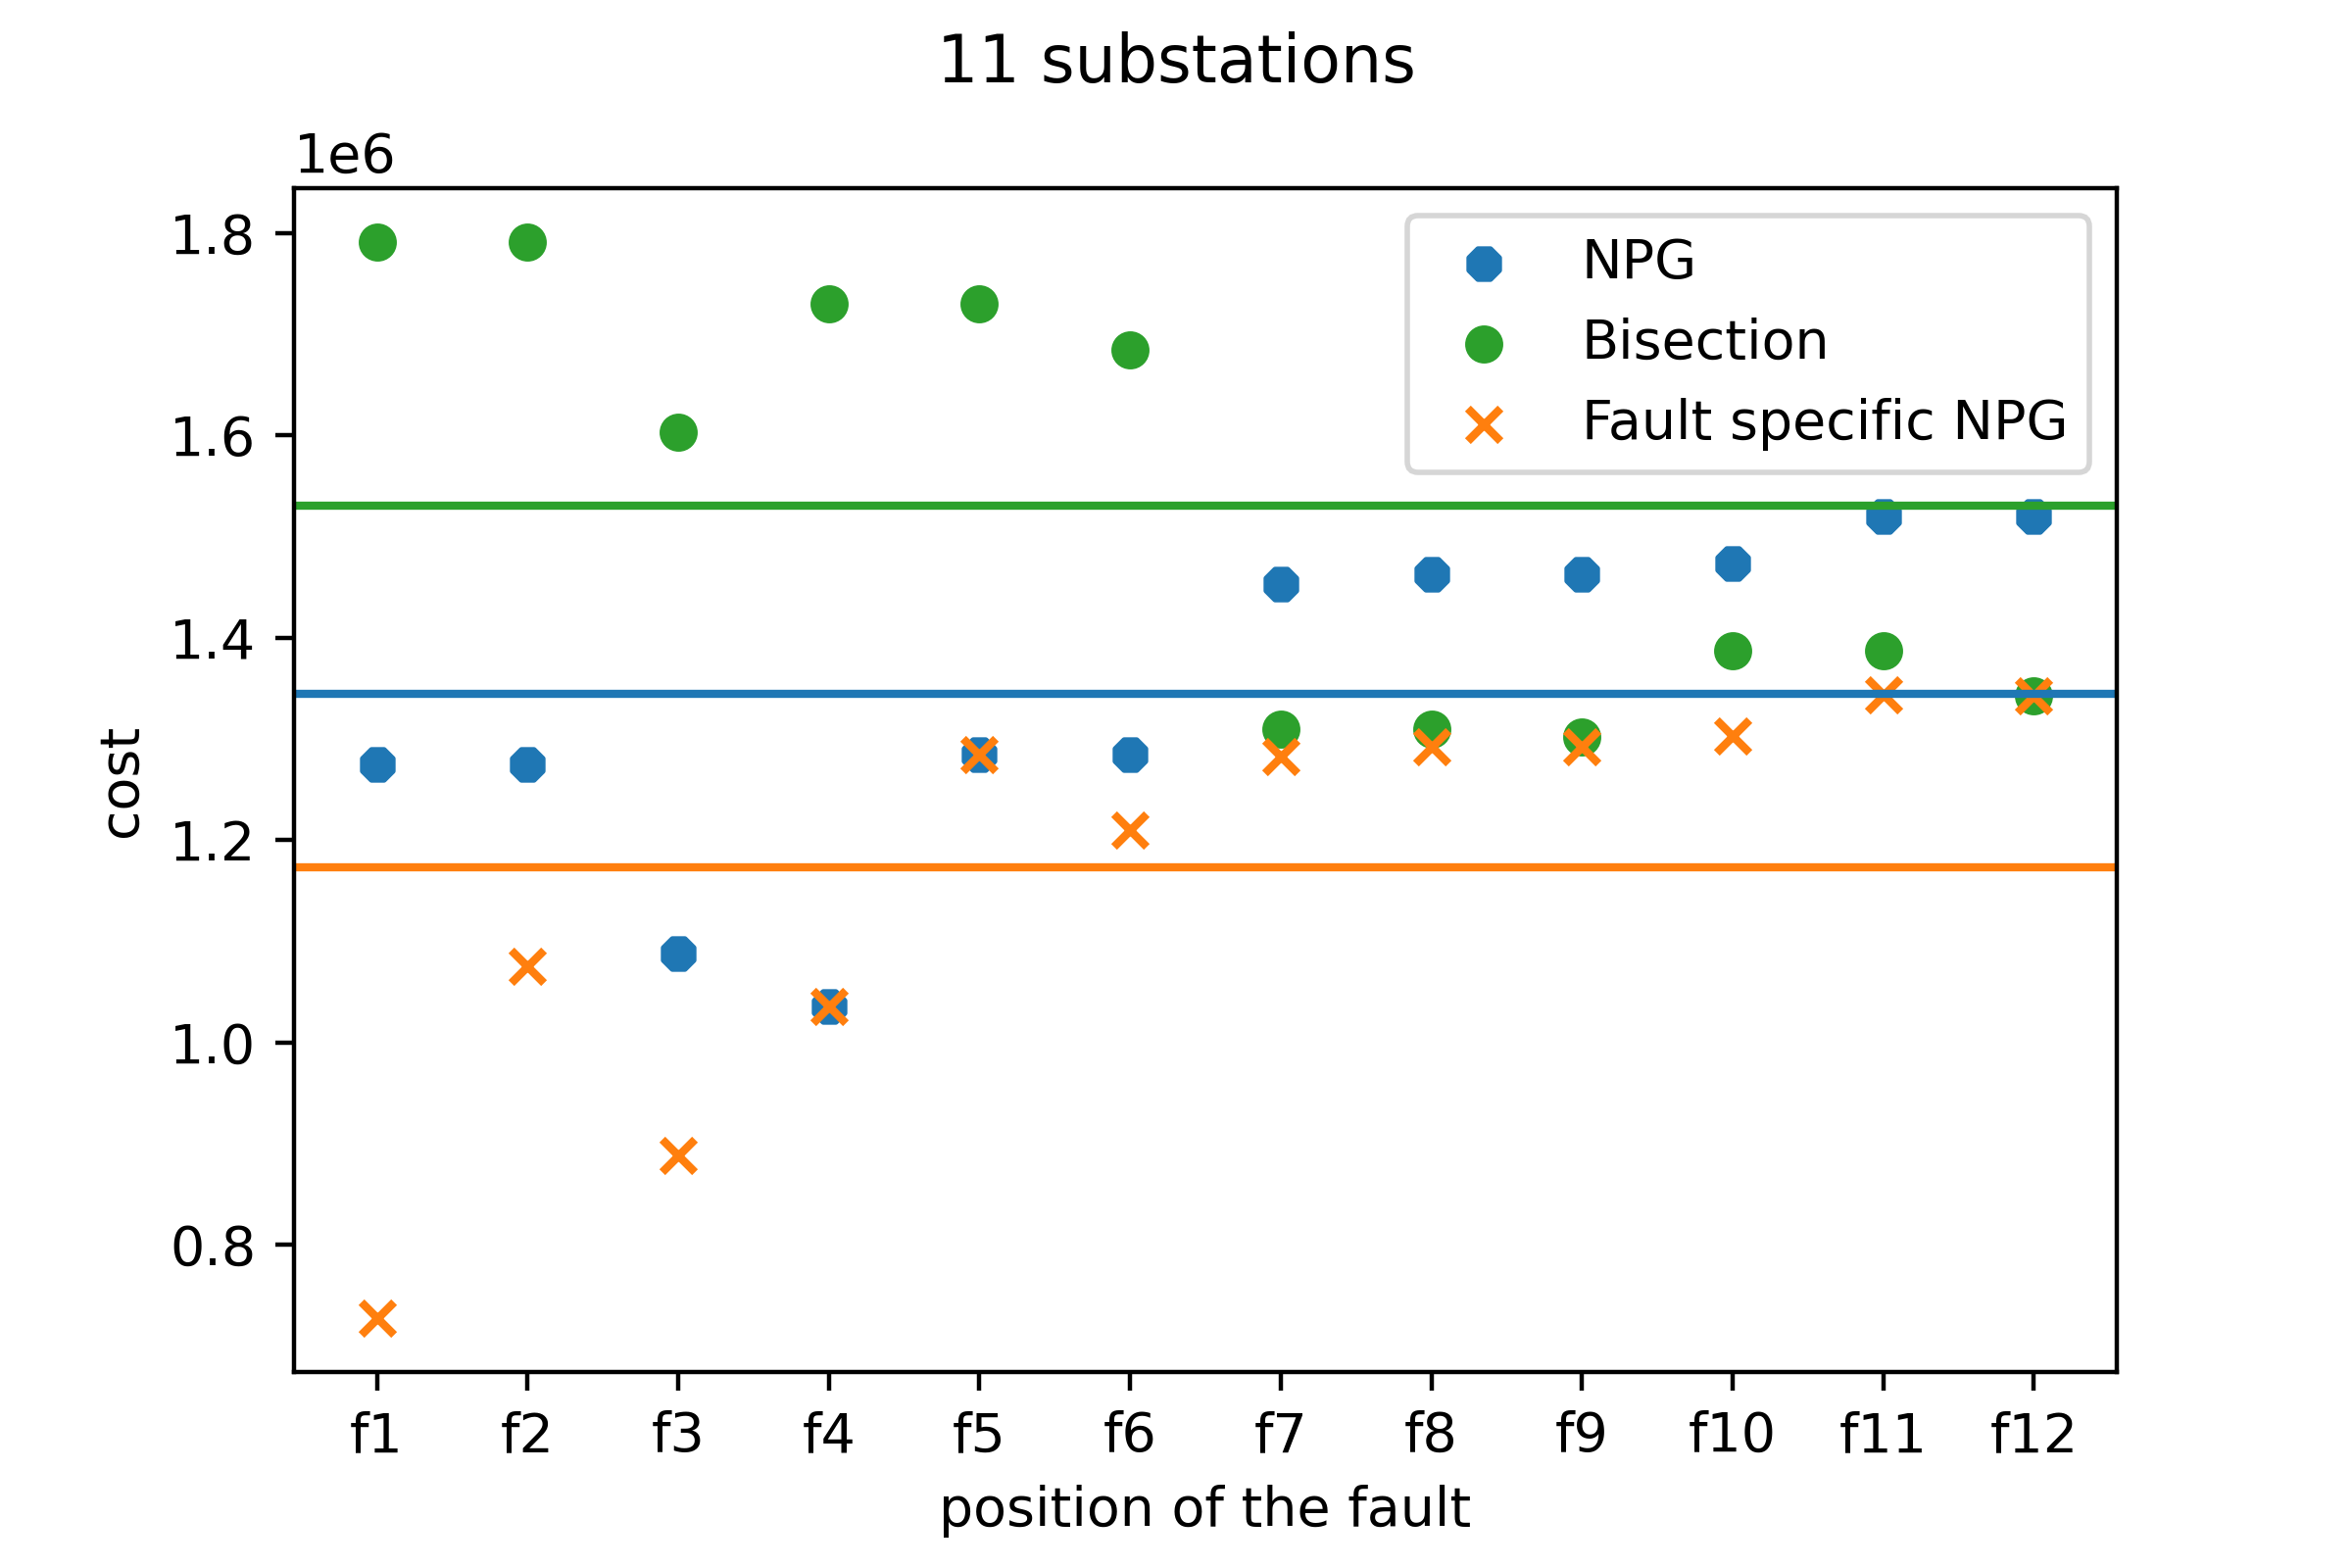
\includegraphics[scale=0.85]{figures/scatterplot.png}
    \end{figure}
    
\end{frame}

\begin{frame}[noframenumbering]{}

    \vspace*{-10pt}
    \begin{figure}
        \centering
        \hspace*{-13pt}
        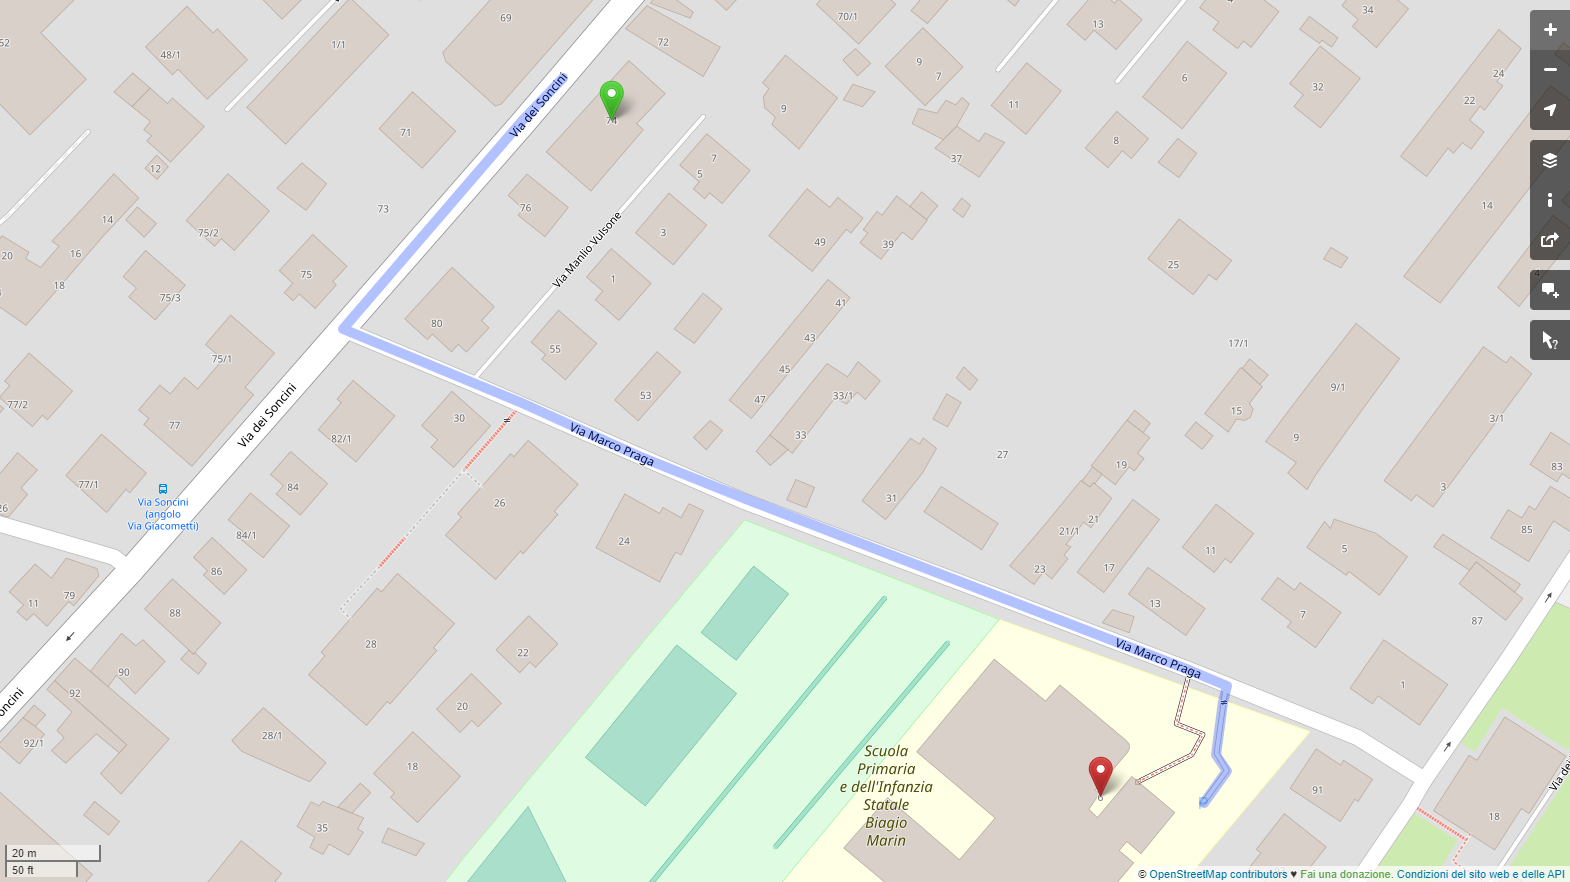
\includegraphics[scale=0.36]{figures/Distanza 7998556-7998442 v2}
    \end{figure}
    
\end{frame}

\begin{frame}[noframenumbering]{}

    \begin{figure}
        \centering
        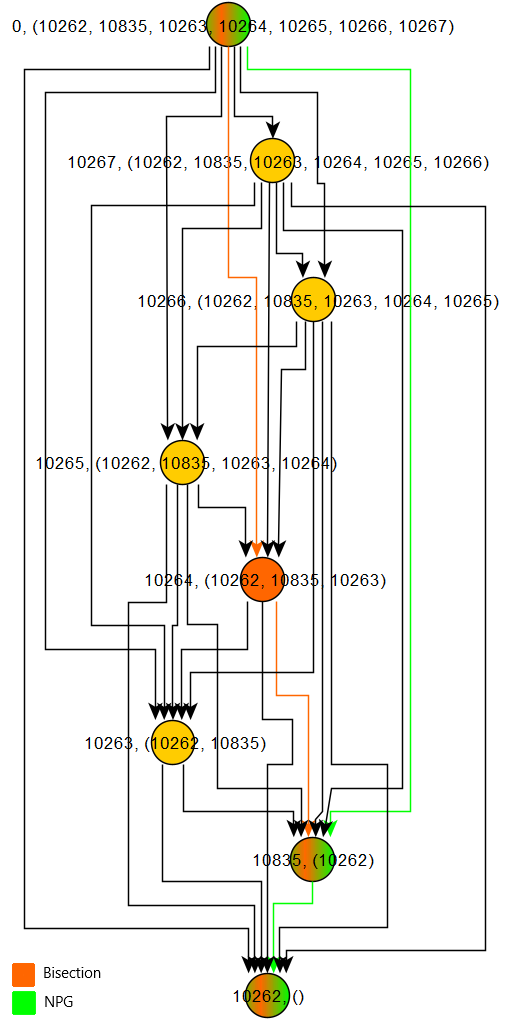
\includegraphics[scale=0.32]{figures/Policies_Bisection_NPG_3}
    \end{figure}
    
\end{frame}


\end{document}